2\vspace*{\fill} % Add flexible vertical space at the top
\begin{center}
    \section*{Declaration of AI use for wording and phrasing}
    AI was used for improved wording and phrasing of the report.
\end{center}
\vspace*{\fill} % Add flexible vertical space at the bottom
\newpage
\tableofcontents

% \newpage
% \textbf{1. Introduction}
% \begin{itemize}
%     \item Motivation: MLIPs for reactive chemistry, limitations of wB97X-D3/6-31G(d) training data (NEB)
%     \item Research questions (DFT-level error, correction strategies)
%     \item Thesis scope and structure
%     \item Research developments
% \end{itemize}

% \textbf{2. Background}
% \begin{itemize}
%     \item Potential energy surfaces and reaction paths
%     \item NEB method (standard + CI-NEB)
%     \item Level of Theory Ladder
%     \begin{itemize}
%     \item OVERALL + Gradient availablity
%     \item DFT functionals and basis sets relevant to this work (wB97X-D3 vs.\ wB97M-V)
%     \item CCSD(T)
%     \item Multireference methods: CASSCF, NEVPT2, AVAS
%     \item Multireference diagnostics: FOD, T1
%     \end{itemize}
%     \item Model Architecture
%     \begin{itemize}
%     \item Graph neural network force fields: PaiNN, MACE
%     \item Delta learning and transfer learning in computational chemistry
%     \end{itemize}
% \end{itemize}

% \textbf{3. Dataset (and Exploratory Analysis)}
% \begin{itemize}
%     \item Transition1x overview (10k reactions, NEB trajectories, wB97X-D3/6-31G(d))
%     \item Chemical diversity: element types, reaction types, barrier distributions
%     \item Comparison with other datasets (QM9x, ANI1x)
%     \item Motivation for higher-level re-evaluation
% \end{itemize}

% \textbf{4. NEB Refinement at wB97M-V/def2-TZVP}
% \begin{itemize}
%     \item Methodology: ORCA, convergence criteria, SLURM workflow
%     \item Results: 174/225 val converged, 279+ test converged
%     \item Barrier comparison: wB97X-D3 vs.\ wB97M-V (systematic shift $\sim$100--200\,meV)
%     \item Failed reactions and handling strategy
% \end{itemize}

% \textbf{6. Multireference Benchmark}
% \begin{itemize}
%     \item FOD screening: method, thresholds, implementation (PySCF, 279 test reactions), 30 reaction with different MR character
%     \item Level-of-theory ladder: wB97X-D3, wB97M-V, CCSD(T)/def2-TZVP, NEVPT2/AVAS/def2-TZVP --- all on identical wB97M-V geometries
%     \item Geometry error vs level of theory error
%     \item CCSD(T) results: barriers for all 30 reactions, triples correction as MR diagnostic
%     \item NEVPT2/AVAS results
%     \item discussing results and takeways
% \end{itemize}

% \textbf{5. Delta Learning}
% \begin{itemize}
%     \item Data selection
%     \item Head architecture
%     \item Results and Comparison (Caveat (no force supervision)
% \end{itemize}


% \textbf{7. Discussion}
% \begin{itemize}
%     \item How large is the DFT-level error and can delta learning fix it?
%     \item Which reactions have genuine MR character and where do SR methods fail?
%     \item Where Can NEVPT2/AVAS serve as standard? (with caveats from red-flag and failed cases) - gap in research
%     \item Interplay between the three threads
% \end{itemize}

% \textbf{8. Conclusion and Future Work}
% \begin{itemize}
%     \item Summary of main findings
% \end{itemize}

% \textbf{Appendix}
% \begin{itemize}
%     \item tbd
% \end{itemize}
% \begin{abstract}
% FILL IN
% \end{abstract}
% \newpage
% \section{Background and Summary}

% Saving computational time
% transition 1x 
% UMA 
% OMOL
% Anatoli
% FILL IN
\chapter{Background}
\label{chap:mr}

\section{Potential Energy Surfaces and Reaction Paths}
\label{sec:background-pes}
\subsection{The Born--Oppenheimer Approximation and the PES}
\label{sec:background-bo}
A molecule is a collection of $N$ nuclei and $n$ electrons interacting through
electrostatic forces. Writing $\mathbf{R} = (\mathbf{R}_1,\dots,\mathbf{R}_N)$ for
the nuclear coordinates and $\mathbf{r} = (\mathbf{r}_1,\dots,\mathbf{r}_n)$ for
the electronic ones, the Hamiltonian in atomic units is
\begin{equation}
\hat{H}
= \underbrace{-\sum_A \frac{\nabla_A^2}{2M_A}}_{\hat{T}_\text{nuc}}
\; \underbrace{- \sum_i \frac{\nabla_i^2}{2}}_{\hat{T}_\text{el}}
\; \underbrace{- \sum_{i,A} \frac{Z_A}{|\mathbf{r}_i - \mathbf{R}_A|}}_{\hat{V}_\text{el-nuc}}
\; \underbrace{+ \sum_{i<j} \frac{1}{|\mathbf{r}_i - \mathbf{r}_j|}}_{\hat{V}_\text{el-el}}
\; \underbrace{+ \sum_{A<B} \frac{Z_A Z_B}{|\mathbf{R}_A - \mathbf{R}_B|}}_{\hat{V}_\text{nuc-nuc}} .
\label{eq:molecular-hamiltonian}
\end{equation}
The two kinetic energy terms and the three Coulomb terms are all that is present.
The difficulty lies in $\hat{V}_\text{el-nuc}$, which couples the electronic and
nuclear coordinates and prevents the eigenvalue problem from separating into
independent electronic and nuclear parts.

A proton is about two thousand times heavier than an electron, and heavier nuclei more so, which makes
$\hat{T}_\text{nuc}$ small compared to $\hat{T}_\text{el}$. Physically, the nuclei
move much more slowly: on the timescale of a bond stretching, the electrons
rearrange many times over, and at any moment they are close to the state they
would occupy if the nuclei were standing still.

\subsubsection*{Fixing the nuclei}
This motivates dropping $\hat{T}_\text{nuc}$ and treating the nuclear coordinates
as fixed numbers rather than dynamical variables. What remains is the electronic
Hamiltonian
\begin{equation}
\hat{H}_\text{el}(\mathbf{R})
= \hat{T}_\text{el} + \hat{V}_\text{el-nuc}(\mathbf{R}) + \hat{V}_\text{el-el}
+ \hat{V}_\text{nuc-nuc}(\mathbf{R}),
\label{eq:electronic-hamiltonian}
\end{equation}
in which $\mathbf{R}$ appears only as a parameter. For each choice of $\mathbf{R}$
this defines a self-contained eigenvalue problem for the electrons alone,
\begin{equation}
\hat{H}_\text{el}(\mathbf{R})\, \psi_k(\mathbf{r};\mathbf{R})
= E_k(\mathbf{R})\, \psi_k(\mathbf{r};\mathbf{R}),
\qquad E_0 \le E_1 \le E_2 \le \dots
\label{eq:electronic-schrodinger}
\end{equation}

\subsubsection*{The potential energy surface}
Only the lowest eigenvalue $E_0(\mathbf{R})$ is needed in what follows. Solving
Eq.~\eqref{eq:electronic-schrodinger} at one geometry gives one number. Solving it
at every geometry gives a function over the whole space of nuclear arrangements,
and this function is the \textbf{potential energy surface} (PES).

\fbox{\begin{minipage}{0.95\linewidth}
\textbf{Key takeaway.} The PES assigns exactly one energy to every possible
arrangement of the atoms --- a scalar function $E : \mathbb{R}^{3N} \to \mathbb{R}$
over the space of nuclear coordinates.
\end{minipage}}
\medskip

For a diatomic molecule there is a single meaningful coordinate, the bond length,
and the PES is a curve with a minimum at the equilibrium geometry. Larger systems
have too many dimensions to plot, but the picture carries over. 
The Born--Oppenheimer approximation is the statement that the nuclei move on this
surface alone. At geometry $\mathbf{R}$ they feel the force
$-\nabla E_0(\mathbf{R})$, and the electrons enter only through the shape of
$E_0$. This holds when the ground state is well separated in energy from the
excited states, which is the case for the reactions studied here.

\subsubsection*{Which surface is actually computed}
Eq.~\eqref{eq:electronic-schrodinger} defines $E_0(\mathbf{R})$ as the lowest
eigenvalue of the electronic Hamiltonian. This is a definition, not a calculation method: the
electronic Schrödinger equation cannot be solved exactly for any molecule with
more than one electron. Approximate methods are used instead --- Hartree--Fock,
Kohn--Sham density functional theory, coupled cluster, CASSCF --- each making
different assumptions about the form the electronic wavefunction is allowed to
take. These are described in Section~\ref{sec:background-electronic}. What matters
here is that every one of them imposes some restriction, and a restriction can
prevent the method from reaching the true ground state at all.

The relevant case here is restricted Kohn--Sham theory, which forces each spatial
orbital to hold one spin-up and one spin-down electron. Some ground states need
the two spins in separate orbitals. Restricted Kohn--Sham keeps them paired and
returns a higher energy. Section~\ref{sec:background-spin} describes when this
happens and why.

The result is a different surface, not merely a shifted one. Its minima and passes
occur at different geometries, and a structure that is a stationary point on the
restricted surface might have a different geometry than a stationary point on the unrestricted one.

\subsection{Stationary Points: Minima and Saddle Points}
\label{sec:background-stationary}

The topology of the PES is characterised by its stationary points, where the
nuclear gradient $\mathbf{g} = \nabla_\mathbf{R} E$ vanishes. The character of a
stationary point is determined by the eigenvalues of the Hessian matrix
$\mathbf{H}_{ij} = \partial^2 E / \partial R_i \partial R_j$:

\begin{itemize}
  \item \textbf{Local minima} ($\mathbf{H}$ positive definite) correspond to
    stable or metastable molecular structures --- reactants and products in
    a chemical reaction.
  \item \textbf{First-order saddle points} (exactly one negative eigenvalue of
    $\mathbf{H}$) correspond to \textbf{transition states} (TS): the highest-energy
    point along the lowest-energy path connecting two minima. The eigenvector
    associated with the single imaginary frequency defines the reaction coordinate
    at the TS.
\end{itemize}

The distinction matters in practice because the two conditions are checked by
different calculations. A vanishing gradient establishes only that a geometry is
\emph{some} stationary point; the number of negative Hessian eigenvalues
establishes \emph{which kind}. A geometry optimisation converges on the former,
and a frequency calculation is required to confirm the latter.

The Hessian is obtained from a frequency calculation. Directions in which the
energy rises give real vibrational frequencies; a direction in which it falls
gives an \emph{imaginary} one. A minimum has none, a transition state exactly one,
and that one mode should be the reaction itself.

The calculation is expensive, and more so when no analytical Hessian is available. It is therefore often
skipped, leaving the character of the located point unverified. This thesis notes
where that is the case.

The energy difference between the transition state and the reactant minimum is the
\textbf{forward barrier height} $\Delta E^\ddagger$; the analogous quantity from
the product side is the \textbf{reverse barrier}. These quantities directly govern
reaction kinetics through transition state theory~\cite{eyring1935}: the rate
constant $k \propto \exp(-\Delta E^\ddagger / k_\text{B} T)$, so errors in
$\Delta E^\ddagger$ translate exponentially into errors in predicted rates.

\subsection{Reaction Paths and the Reaction Coordinate}
\label{sec:background-reactionpath}

A \textbf{reaction path} is a one-dimensional curve on the PES connecting the
reactant minimum to the product minimum through the transition state. The
standard definition is the \textbf{intrinsic reaction coordinate} (IRC), introduced by Fukui~\cite{fukui1981}: the steepest descent path from the transition
state down to both minima, computed in coordinates scaled by atomic mass so that
the path is the one a classical particle would follow.

The energy profile $E(s)$ along the MEP has a single maximum at the transition state
and minima at the endpoints. This property is computed, compared, and predicted throughout this thesis.

\subsection{Separating Geometry and Energy on the PES}
\label{sec:geom-energy}

Although the PES is a single object, every electronic structure calculation reports
two logically distinct things: a nuclear \emph{geometry} --- a point in
$\mathbb{R}^{3N}$, such as the location of a saddle point --- and a scalar
\emph{energy} --- the height of the PES at that point. A barrier height combines
both: it is the energy at the transition-state geometry, measured relative to the
reactant. The accuracy of a computed barrier therefore depends on two contributions
that can fail independently: the accuracy of the transition-state \emph{geometry}
and the accuracy of the \emph{energy} evaluated at that geometry.

The two are separable in practice. A geometry optimised with one method can be
handed to another method for an energy evaluation --- a \emph{single-point}
calculation. This is standard, and often unavoidable, since the most accurate
methods have no affordable gradients and cannot optimise a geometry at all
(Section~\ref{sec:background-ladder}). A reference calculation therefore has two
levels, not one: a geometry level and an energy level.

The separation also splits the diagnosis. A method can give the wrong energy at
the right geometry, or place the stationary point at the wrong geometry, and the
two are answered by different tests: one asks for the energy at a fixed point, the
other asks where the gradient vanishes.

\subsection{Relevance to Machine Learning Potentials}
\label{sec:background-mlip-relevance}

An MLIP approximates $E(\mathbf{R})$ directly as a parametric function of atomic
positions, bypassing the electronic Schrödinger equation entirely. It has no
wavefunction and no access to the electronic structure --- only the surface its
training labels trace out. The Transition1x data used in this work was generated at
the \mbox{wB97X-D3/6-31G(d)} level, and the resulting errors in barrier heights are
what Chapter~\ref{ch:delta} sets out to correct.
Section~\ref{sec:background-mlip} develops all of this properly.

% ─────────────────────────────────────────────────────────────
\section{The Nudged Elastic Band Method}
\label{sec:background-neb}

\subsection{The Transition State Problem}

Locating the transition state of a chemical reaction requires finding a first-order
saddle point on the PES that connects two known minima. This is inherently more
difficult than minimisation: gradient-based optimisers naturally descend toward
minima, and following the gradient away from a saddle point is numerically
unstable. The difficulty is compounded by the high dimensionality of the PES ---
a molecule with $N$ atoms has $3N - 6$ internal degrees of freedom, and the TS
may be far from both endpoints in this space. A double-ended method, which uses
knowledge of both reactant and product geometries to guide the search, is therefore
more practical than a single-ended method that searches blindly from the reactant.

\subsection{NEB: Minimum Energy Path as a Discretised Chain}

The nudged elastic band (NEB) method~\cite{jonsson1998, henkelman2000tangent}
finds the minimum energy path (MEP) between two known structures by representing
the path as a discrete chain of $N_\text{img}$ images $\{\mathbf{R}_0, \mathbf{R}_1,
\ldots, \mathbf{R}_{N_\text{img}-1}\}$, where $\mathbf{R}_0$ and
$\mathbf{R}_{N_\text{img}-1}$ are fixed at the reactant and product geometries.
The images are connected by fictitious elastic springs that maintain an even spacing
along the path, while each image is simultaneously relaxed toward the true MEP. The
key insight of the NEB method is the \textbf{nudging} projection: the spring force
is projected to act only along the path tangent (preventing the chain from shortcutting
the barrier), and the true PES gradient is projected to act only perpendicular to the
tangent (preventing the images from sliding to the minima). Formally, the force on
image $i$ is:

\begin{equation}
  \mathbf{F}_i = -\nabla E(\mathbf{R}_i)\big|_\perp + \mathbf{F}_i^\text{spring}\big|_\parallel,
\end{equation}

where $\perp$ and $\parallel$ denote components perpendicular and parallel to the
local path tangent $\hat{\boldsymbol{\tau}}_i$. The spring force along the tangent
is $\mathbf{F}_i^\text{spring}\big|_\parallel = k(|\mathbf{R}_{i+1} - \mathbf{R}_i|
- |\mathbf{R}_i - \mathbf{R}_{i-1}|)\hat{\boldsymbol{\tau}}_i$, where $k$ is the
spring constant. Convergence is reached when the perpendicular gradient component
falls below a threshold $f_\text{max}$ for all images.

\subsection{CI-NEB: Converging on the Saddle Point}

The standard NEB gives a discretised MEP but does not in general place any image
exactly at the saddle point --- the transition state lies between two images.
The \textbf{climbing image} modification (CI-NEB~\cite{henkelman2000cineb}) remedies
this by identifying the highest-energy image and modifying its force so that it
climbs uphill along the path while relaxing perpendicular to it:

\begin{equation}
  \mathbf{F}_i^\text{CI} = -\nabla E(\mathbf{R}_i) +
  2\,\nabla E(\mathbf{R}_i)\big|_\parallel.
\end{equation}

The spring force is removed entirely for the climbing image, and the parallel
component of the true gradient is inverted, driving the image toward the saddle
point. CI-NEB therefore converges on a first-order saddle point of the surface it
is run on, giving both a transition state geometry and an estimate of the barrier
height from the energy profile of the full band. 
(Section~\ref{sec:background-spin}).

\subsection{NEB in This Work}

NEB is used in two distinct roles in this thesis. First, the Transition1x dataset
was generated by running NEB at the \mbox{wB97X-D3/6-31G(d)} level to produce
approximately 10\,000 reaction paths, providing training data for MACE and PaiNN.
Second, another set (Transition1x testset) of reactions was re-run at the higher
\mbox{wB97M-V/def2-TZVP} level using ORCA~5 via the ASE interface, providing
refined geometries and energies for benchmarking. In both cases, CI-NEB with 10
images per band was used, with convergence defined as $f_\text{max} <
0.05$\,eV/\AA{} for the climbing image.

The broader goal of this project is to replace the DFT calculator in the NEB loop
with a trained MLIP entirely. Rather than computing energies and forces with an
expensive quantum chemistry program at each optimisation step, the MLIP would serve
as the calculator directly --- reducing the cost of a full NEB from hours of DFT to
seconds of inference. All model developments in this thesis are therefore benchmarked
in the context of NEB: the quality of a model is assessed not only by its energy and
force errors on single fixed geometries, but by the barrier heights and transition state
geometries it produces when driving NEB independently. Comparisons are made against
state-of-the-art foundation models trained on the \mbox{wB97M-V/def2-TZVPD}
Open Molecules 2025 (OMol25) dataset~\cite{omol25}: the eSEN
architecture~\cite{esen} and the Universal Model for Atoms
(UMA)~\cite{uma}, both released by Meta FAIR in 2025. These models represent the
current frontier of general-purpose MLIPs for organic chemistry and serve as
external baselines for the NEB-driven benchmarks.

\section{Electronic Structure Methods}
\label{sec:background-electronic}

An electronic structure method computes $E(\mathbf{R})$: given the nuclear
positions, it returns the energy of the electrons and the gradient that follows
from it. Every point on a potential energy surface comes from one such
calculation. Doing this exactly is impossible beyond one electron, so every method
restricts the form the wavefunction is allowed to take, and trades accuracy
against cost. Where the true ground state falls outside the form a method allows,
it returns something else without indicating that it has.

\subsection{Single-Reference versus Multireference Electronic Structure}
\label{sec:sr-vs-mr}

Section~\ref{sec:background-bo} introduced the question of which surface an
approximate method returns. Answering it requires two terms.

Electrons are described by \textbf{orbitals}: one-electron functions, each holding
at most two electrons of opposite spin. A \textbf{configuration} is one particular
assignment of all the electrons to orbitals --- which are occupied, which are
empty. Written out as a wavefunction, one configuration is one \textbf{Slater
determinant} $\Phi_I$, the determinant form being what enforces the antisymmetry
the Pauli principle requires.

Any electronic state can be written as a weighted sum of such determinants,
%
\begin{equation}
  \Psi = \sum_I c_I \, \Phi_I ,
  \qquad \sum_I |c_I|^2 = 1 ,
  \label{eq:ci-expansion}
\end{equation}
%
where $|c_I|^2$ is the weight of configuration $I$. How this weight is distributed
splits the problem into two regimes.

\paragraph{Single-reference regime.}
At most geometries one configuration carries nearly all the weight,
$|c_0|^2 \approx 1$, and every other term in Equation~\ref{eq:ci-expansion} is a
small correction to it. Methods built on one dominant configuration ---
Hartree--Fock, density functional theory, coupled cluster --- work well here. It is
the regime they were designed for.

\paragraph{Multireference regime.}
Near bond breaking, at diradical intermediates and at many transition states, two
or more coefficients become comparable in size. Consider a bond halfway broken.
Its two electrons can still be described as a pair sharing one orbital, or as one
electron on each of the two separating atoms. Both configurations cost roughly the
same energy, so both carry substantial weight, and no single determinant captures
the state.

Two responses exist. Build the reference from several determinants at once and
optimise their coefficients explicitly (Section~\ref{sec:background-mr}), or keep
a single determinant and lift the constraint that forces the two electrons to
share an orbital (Section~\ref{sec:background-spin}). The second reaches similar
energies far more cheaply, and gives up a formal property of the wavefunction in
exchange. It is the route used in this thesis.

\paragraph{Consequence for the geometry--energy separation.}
The question has to be asked twice, since a reference calculation has a geometry
level and an energy level (Section~\ref{sec:geom-energy}): the method that finds
the saddle point must be adequate, and so must the method that evaluates the
energy there. Common practice assumes they need not be equally good. Structures
are held to be far less sensitive to the functional and basis set than
energies~\cite{bursch2022}, which is what justifies optimising cheaply and then
computing a single-point energy at a higher level. On that reasoning a
single-reference method could place the saddle point correctly even where its
energy at that point is systematically wrong.

The reasoning holds as long as the single-reference calculation describes the
electronic ground state. Chapter~\ref{ch:mr} examines what happens where it does
not.

% ─────────────────────────────────────────────────────────
\subsection{Density Functional Theory}
\label{sec:background-dft}

\subsubsection{The Many-Body Problem and the Key Insight of DFT}

Solving the electronic Schrödinger equation exactly for a molecule with $N_e$
electrons requires knowing the full many-body wavefunction
$\Psi(\mathbf{r}_1, \ldots, \mathbf{r}_{N_e})$ --- a function of $3N_e$ spatial
coordinates. For even a modest molecule of 20 electrons this is a function in 60
dimensions, and the computational cost of exact diagonalisation grows
exponentially with $N_e$. No practical calculation is possible beyond a handful
of electrons.

Density functional theory (DFT) offers a radical simplification. The
Hohenberg--Kohn theorems (1964) prove that the ground-state energy of an
electronic system is a unique functional of the electron density
$\rho(\mathbf{r})$ alone --- a function of just three spatial coordinates,
regardless of the number of electrons. Knowing $\rho(\mathbf{r})$ is in principle
sufficient to determine everything about the ground state. The many-body problem
in $3N_e$ dimensions collapses to a problem in 3 dimensions.

\subsubsection{The Kohn--Sham Approach and the Exchange--Correlation Functional}

In practice, the exact density functional is unknown. Kohn and Sham (1965)
reformulated the problem by introducing a fictitious system of \emph{non-interacting}
electrons moving in an effective potential chosen so that their density exactly
matches the true interacting density. The non-interacting electrons occupy
single-particle orbitals $\phi_i(\mathbf{r})$ (the Kohn--Sham orbitals), and
the total energy is:

\begin{equation}
  E[\rho] = T_s[\rho] + E_\text{ext}[\rho] + E_\text{Hartree}[\rho]
            + E_\text{XC}[\rho],
\end{equation}

where $T_s$ is the kinetic energy of the non-interacting electrons, $E_\text{ext}$
is the electron--nuclear attraction, $E_\text{Hartree}$ is the classical
electron--electron repulsion, and $E_\text{XC}$ --- the
\textbf{exchange--correlation (XC) functional} --- captures everything else:
quantum mechanical exchange, electron correlation, and the correction to the
kinetic energy from the real interacting system. The first three terms are computed
exactly. Only $E_\text{XC}$ must be approximated.

The Kohn--Sham equations are solved iteratively, because the effective potential
in which the orbitals move depends on the density that those same orbitals
produce. Starting from an initial guess for the orbitals, one constructs the
effective potential, solves for a new set of orbitals, forms the new density, and
repeats until the density no longer changes --- the \textbf{self-consistent
field} (SCF) procedure. The converged result is a stationary point of the energy
with respect to variation of the orbitals. Two properties of this procedure
matter later: the outcome can depend on the initial guess, since the iteration
converges to whichever stationary point it is drawn towards; and a converged
solution is stationary but not necessarily the lowest one, a distinction taken up
in Section~\ref{sec:background-stability}.

The exchange--correlation functional is the central approximation in DFT, and
the accuracy of any DFT calculation depends almost entirely on the quality of
this approximation. Decades of development have produced a hierarchy of increasingly
sophisticated approximations, commonly organised on \textbf{Jacob's ladder}
(Figure~\ref{fig:jacobs-ladder}), ascending from crude local approximations to
highly accurate nonlocal ones.

\begin{figure}[h]
\centering
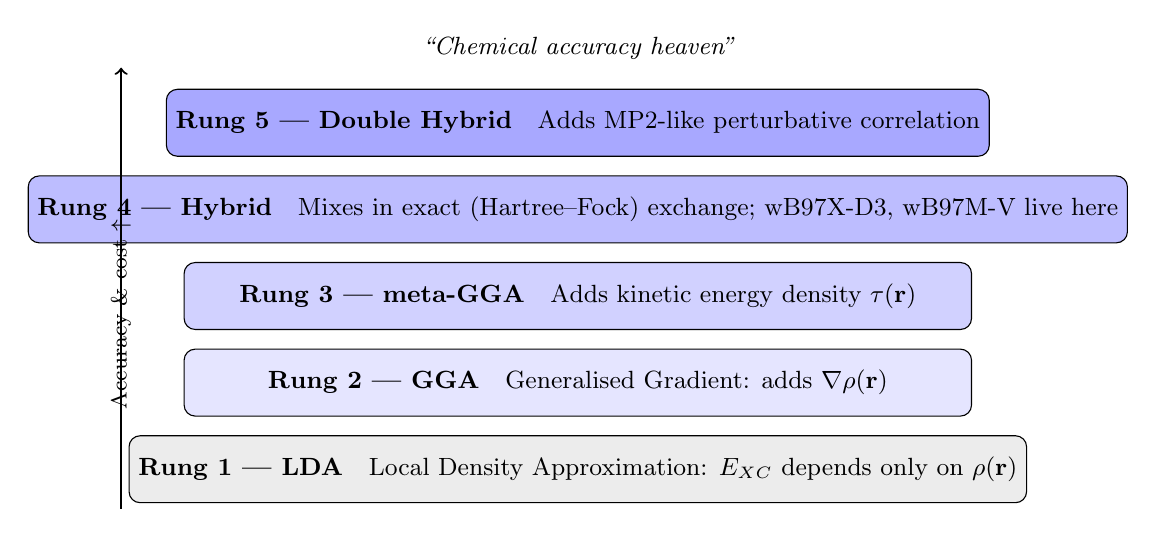
\begin{tikzpicture}[
  rung/.style={draw, rounded corners=4pt, fill=#1, minimum width=10cm,
               minimum height=0.85cm, align=center, font=\small},
  lbl/.style={font=\footnotesize, align=left, text width=4.5cm},
]
% Rungs bottom to top
\node[rung=gray!15]    (r1) at (0,0.00) {\textbf{Rung 1 — LDA}\quad
  Local Density Approximation: $E_\text{XC}$ depends only on $\rho(\mathbf{r})$};
\node[rung=blue!10]    (r2) at (0,1.10) {\textbf{Rung 2 — GGA}\quad
  Generalised Gradient: adds $\nabla\rho(\mathbf{r})$};
\node[rung=blue!18]    (r3) at (0,2.20) {\textbf{Rung 3 — meta-GGA}\quad
  Adds kinetic energy density $\tau(\mathbf{r})$};
\node[rung=blue!26]    (r4) at (0,3.30) {\textbf{Rung 4 — Hybrid}\quad
  Mixes in exact (Hartree--Fock) exchange; \mbox{wB97X-D3}, \mbox{wB97M-V} live here};
\node[rung=blue!34]    (r5) at (0,4.40) {\textbf{Rung 5 — Double Hybrid}\quad
  Adds MP2-like perturbative correlation};

% Heaven label
\node[font=\small\itshape] at (0, 5.35) {``Chemical accuracy heaven''};

% Arrow on the left
\draw[->, thick] (-5.8,-0.5) -- (-5.8,5.1)
  node[midway, left, font=\footnotesize, align=center, rotate=90,
       xshift=1cm] {Accuracy \& cost $\uparrow$};

\end{tikzpicture}
\caption{Jacob's ladder of density functional approximations. Each rung adds
more physical ingredients to the exchange--correlation functional, generally
increasing accuracy at the cost of computational expense. Both functionals used
in this thesis sit on Rung~4: \mbox{wB97X-D3} as a hybrid GGA and \mbox{wB97M-V}
as a hybrid meta-GGA.}
\label{fig:jacobs-ladder}
\end{figure}

\subsubsection{Hybrid Functionals and Range Separation}

Rung~4 hybrid functionals improve upon lower rungs by mixing a fraction of
\emph{exact exchange} --- the exchange energy computed from the Kohn--Sham
orbitals as in Hartree--Fock theory --- into the approximate XC functional.
This reduces self-interaction error and generally improves barrier heights, which
are systematically underestimated by GGA and meta-GGA functionals.

\textbf{Range-separated} hybrids go further by splitting the electron--electron
interaction into short-range and long-range components using a partitioning
parameter $\omega$:
%
\begin{equation}
  \frac{1}{r_{12}} = \underbrace{\frac{1-\text{erf}(\omega r_{12})}{r_{12}}}_{\text{short range (DFT)}}
  + \underbrace{\frac{\text{erf}(\omega r_{12})}{r_{12}}}_{\text{long range (HF exchange)}}.
\end{equation}
%
At short range, the DFT exchange approximation is accurate. At long range, exact
exchange is used instead, correctly describing charge-transfer interactions and
improving the asymptotic behaviour of the potential. The $\omega$B97 family of
functionals exploits this splitting.

\textbf{Dispersion corrections} address a further weakness of standard DFT: the
inability to describe van der Waals (London dispersion) interactions, which arise
from correlated fluctuations in electron density and are entirely absent from local
XC approximations. The D3 correction~\cite{grimme2010} adds atom-pairwise damped
$C_6/r^6$ terms to the DFT energy; the VV10 non-local correlation
functional~\cite{vydrov2010} takes a more principled approach by computing
dispersion from a double integral over the electron density. Both approaches
correct the same physics; VV10 is generally more accurate for strongly interacting
pairs.

\subsubsection{The Two Functionals in This Work}

\textbf{\mbox{wB97X-D3/6-31G(d)}}~\cite{lin2013} is a range-separated hybrid
GGA with D3 pairwise dispersion. It was chosen for generating Transition1x due to
its good overall performance and affordable cost. Its main limitations for this
thesis are the small basis set (discussed below) and the absence of kinetic energy
density (a Rung~3 ingredient), which limits its accuracy for barrier heights
relative to meta-GGA functionals.

\textbf{\mbox{wB97M-V/def2-TZVP}}~\cite{mardirossian2016} is a range-separated
hybrid \emph{meta}-GGA with VV10 non-local dispersion. The additional kinetic
energy density ingredient adds a Rung~3 ingredient the other functional lacks, and
VV10 is more physically rigorous than pairwise D3 for dispersion. In the
comprehensive GMTKN55 benchmark~\cite{goerigk2017}, \mbox{wB97M-V} consistently
ranks among the most accurate Rung~4 functionals for thermochemistry, kinetics,
and non-covalent interactions. It is used as the NEB refinement level and the
target level for the delta learning approach in this thesis.

% ─────────────────────────────────────────────────────────
\subsection{Basis Sets}
\label{sec:background-basis}

\subsubsection{Representing Molecular Orbitals}

A Kohn--Sham orbital $\phi_i(\mathbf{r})$ is a function of continuous space.
To make it computable, it must be represented in a finite set of known
functions --- a \textbf{basis set}. The standard approach (LCAO: linear combination
of atomic orbitals) expresses each molecular orbital as a sum over atom-centred
basis functions $\chi_\mu$:

\begin{equation}
  \phi_i(\mathbf{r}) = \sum_\mu c_{\mu i}\, \chi_\mu(\mathbf{r} - \mathbf{R}_A),
\end{equation}

where $\mathbf{R}_A$ is the position of atom $A$ and the coefficients $c_{\mu i}$
are determined variationally. In practice, each basis function $\chi_\mu$ is a
\textbf{contracted Gaussian-type orbital} (GTO): a fixed linear combination of
Gaussian functions $e^{-\alpha_k |\mathbf{r}|^2}$ with different exponents
$\alpha_k$, centred on the atom. Gaussians are used because integrals of products
of Gaussians can be evaluated analytically, making the construction of the Kohn--Sham
matrix efficient.

The key parameters of a basis set are its \textbf{size} (how many basis functions
per atom) and its \textbf{composition} (which angular momentum types are included).
Larger basis sets represent the orbital more accurately but increase computational
cost as $\mathcal{O}(N_\text{basis}^4)$ for DFT. Figure~\ref{fig:basis-sets}
illustrates the two basis sets used in this thesis.

\begin{figure}[h]
\centering
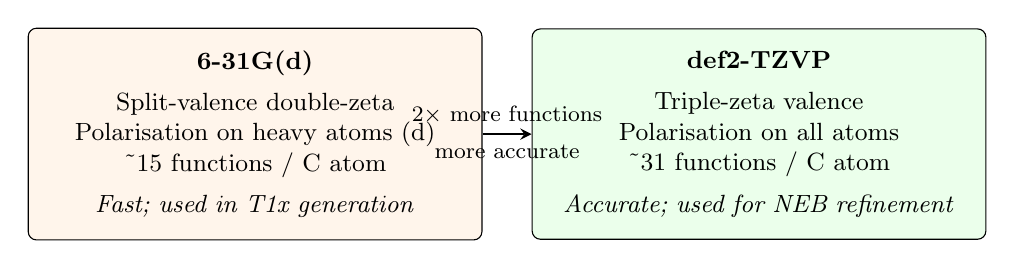
\begin{tikzpicture}[
  box/.style={draw, rounded corners=3pt, align=center, minimum height=2.2cm,
              text width=5.2cm, font=\small, inner sep=8pt},
  arr/.style={->, thick, >=stealth},
]

\node[box, fill=orange!8] (small) at (-3.2,0) {
  \textbf{6-31G(d)} \\[4pt]
  Split-valence double-zeta \\
  Polarisation on heavy atoms (d) \\
  \textasciitilde 15 functions / C atom \\[4pt]
  \textit{Fast; used in T1x generation}
};

\node[box, fill=green!8] (large) at (3.2,0) {
  \textbf{def2-TZVP} \\[4pt]
  Triple-zeta valence \\
  Polarisation on all atoms \\
  \textasciitilde 31 functions / C atom \\[4pt]
  \textit{Accurate; used for NEB refinement}
};

\draw[arr] (small.east) -- (large.west)
  node[midway, above, font=\footnotesize] {$2\times$ more functions}
  node[midway, below, font=\footnotesize] {more accurate};

\end{tikzpicture}
\caption{The two basis sets used in this thesis. A larger, more complete basis
set reduces the \emph{basis set incompleteness error} at increased computational
cost.}
\label{fig:basis-sets}
\end{figure}

\subsubsection{Reading a Method Specification: wB97X-D3/6-31G(d)}

A method specification like \mbox{wB97X-D3/6-31G(d)} encodes two independent
choices separated by a slash: the \textbf{functional} (wB97X-D3) and the
\textbf{basis set} (6-31G(d)). The functional determines how electron--electron
interactions are approximated; the basis set determines how the orbitals are
represented. Both introduce errors independently, and both are addressed in this
thesis: the functional by switching from wB97X-D3 to wB97M-V (higher rung on
Jacob's ladder), and the basis set by switching from 6-31G(d) to def2-TZVP
(more functions, better description).

A method specification of this form is nonetheless incomplete. It records two of
the three choices that define a Kohn--Sham calculation; the third --- the spin
ansatz --- is the subject of the following section.

% ─────────────────────────────────────────────────────────
\subsection{Spin Formalism: Restricted, Unrestricted, and Broken Symmetry}
\label{sec:background-spin}

Sections~\ref{sec:background-dft} and \ref{sec:background-basis} specified two of
the three choices that define a Kohn--Sham calculation: the functional and the
basis set. A third choice is made every time, but is rarely stated, because in
most cases it is made by the program rather than by the user: the constraint
imposed on the spin orbitals.

\subsubsection{Three Ansätze}

The Kohn--Sham orbitals introduced in Section~\ref{sec:background-dft} carry a
spin label in addition to their spatial part. Three treatments are in common use.

\textbf{Restricted Kohn--Sham (RKS)} constrains $\alpha$ and $\beta$ electrons to
occupy the \emph{same} spatial orbitals, so that every occupied orbital holds
exactly one electron pair,
%
\begin{equation}
  \phi_i^\alpha(\mathbf{r}) = \phi_i^\beta(\mathbf{r}) \quad \forall i .
\end{equation}
%
The resulting density is a spin eigenfunction by construction, $\langle S^2
\rangle = 0$ for a singlet, and the calculation is roughly half as expensive as
the unrestricted one because only one set of orbitals is optimised.

\textbf{Unrestricted Kohn--Sham (UKS)} lifts this constraint and optimises
$\phi_i^\alpha$ and $\phi_i^\beta$ independently. The additional variational
freedom means that the UKS energy is always less than or equal to the RKS energy
at the same geometry. The price is that the resulting determinant need not be a
spin eigenfunction: $\langle S^2 \rangle$ may deviate from its formal value, an
effect known as \emph{spin contamination}.

The expectation value $\langle S^2 \rangle$ measures this deviation and is
reported by every unrestricted calculation. Its exact values are $S(S+1)$, so
$0$ for a singlet, $2$ for a triplet. A restricted singlet returns $\langle S^2
\rangle = 0$ by construction. An unrestricted singlet solution with $\langle S^2
\rangle$ between these values is a mixture: $\langle S^2 \rangle \approx 1$
corresponds to roughly equal singlet and triplet character, the value expected
for two electrons localised on separate centres with no coupling. The magnitude
therefore serves as a direct indicator of how far a given solution has departed
from spin purity.

\textbf{Broken-symmetry (BS) solutions} are the physically interesting subset of
UKS solutions for singlets. If two electrons localise on separate centres with
opposite spin, the $\alpha$ and $\beta$ densities differ in space while the total
spin remains zero. Such a solution has $\langle S^2 \rangle$ between $0$ and $1$
and is, formally, an approximately equal mixture of singlet and triplet. It is
not a spin-pure wavefunction, but it captures the energetics of an open-shell
singlet at the cost of a single-determinant calculation.

\subsubsection{Multiplicity Does Not Determine the Occupation}

The input to a calculation specifies the charge and the spin multiplicity. For a
neutral organic molecule with an even number of electrons this is $0$ and $1$.
Multiplicity one states only that the total spin is zero, and two physically
distinct situations satisfy that condition:

\begin{itemize}
  \item a \textbf{closed-shell} molecule, in which each occupied orbital holds an
    electron pair;
  \item an \textbf{open-shell singlet} (a biradical), in which two electrons
    occupy separate orbitals with opposite spin.
\end{itemize}

From the input alone the two are indistinguishable, and this is the reason the
choice of ansatz is usually made by the program. Every major code selects a
restricted treatment for a closed-shell singlet input unless instructed otherwise.
The ORCA manual states that ``for closed-shell molecules with multiplicity 1,
RHF/RKS is assumed''~\cite{orca_manual}; PySCF dispatches to \texttt{RKS} whenever
\texttt{mol.spin == 0}~\cite{pyscf}; the \texttt{UNRESTRICTED} keyword in Q-Chem
defaults to \texttt{FALSE}~\cite{qchem_manual}; the Psi4 \texttt{REFERENCE}
keyword defaults to RHF~\cite{psi4}; NWChem documents that ``SINGLET is the
default, and specifies a closed shell''~\cite{nwchem}.

The restricted ansatz is appropriate for the first situation and not for the
second. The Q-Chem manual makes the distinction explicitly, noting that a
restricted treatment is ``typically appropriate for closed shell molecules at
their equilibrium geometry'' while an unrestricted one is appropriate ``for
molecules with even numbers of electrons where not all electrons are paired,
e.g., stretched bonds and diradicals''~\cite{qchem_manual}. The qualifier matters:
it is the equilibrium geometry, not the molecule, that makes the restricted
treatment appropriate.

\fbox{\begin{minipage}{0.95\linewidth}
\textbf{Key takeaway.} Multiplicity one is consistent with both a closed-shell
molecule and an open-shell singlet. The restricted ansatz assumes the former;
where the latter holds, it describes a higher-lying state.
\end{minipage}}

\medskip
Transition states of bond-breaking reactions are precisely the geometries at
which the second situation arises: as a bond is broken, an electron pair
separates onto two centres. The best-practice review of Bursch \emph{et
al.}~\cite{bursch2022} names ``transition states of open-shell dissociation
processes'' among the cases for which multireference character should be
expected, and recommends checking such systems with an unrestricted
broken-symmetry calculation. This makes the choice of ansatz a substantive part
of the definition of a reference calculation, on the same footing as the
functional and the basis set, and it is why Chapter~\ref{ch:mr} treats it
explicitly.

\subsubsection{Symmetry Must Be Broken Deliberately}

Specifying an unrestricted calculation is necessary but not sufficient to obtain
a broken-symmetry solution. The restricted solution is itself a stationary point
of the unrestricted energy functional: if the initial guess is spin-symmetric,
the SCF procedure has no gradient along the symmetry-breaking direction and
converges back to it. Obtaining a broken-symmetry solution therefore requires
perturbing the initial guess --- commonly by mixing the $\beta$ HOMO and LUMO
through a finite rotation, by a spin-flip on one fragment, or by following the
instability direction identified by the analysis described below.

This asymmetry is what makes the practical recommendation simple. An unrestricted
calculation started from a symmetry-broken guess converges to a broken-symmetry
solution where one exists, and back to the restricted solution where none does.
A restricted calculation can only ever return the restricted solution. Using an
unrestricted ansatz therefore costs nothing where the restricted solution is
correct, and is the only route to the correct solution where it is not.

% ─────────────────────────────────────────────────────────
\subsection{SCF Stability Analysis}
\label{sec:background-stability}

Whether a lower solution exists at a given geometry is decided by an SCF
stability analysis. The self-consistent field procedure converges to a stationary
point of the energy with respect to orbital rotations, but a stationary point is
not necessarily a minimum. The analysis constructs the electronic Hessian --- the
second derivative of the energy with respect to orbital rotation parameters ---
and examines its lowest eigenvalues.

Two directions are distinguished, in analogy with the nuclear Hessian of
Section~\ref{sec:background-stationary} but in orbital rather than nuclear space:

\begin{itemize}
  \item \textbf{Internal stability} asks whether a lower solution exists
    \emph{within the same ansatz}. A negative eigenvalue means the SCF has
    converged to a saddle point in orbital space rather than to a minimum, and
    the calculation should be reconverged.
  \item \textbf{External stability} asks whether a lower solution exists in the
    \emph{next larger} class of wavefunctions. For a restricted solution the
    relevant extension is the unrestricted one: a negative external eigenvalue
    $\lambda_\mathrm{ext}$ means that a broken-symmetry solution lies below the
    restricted one, so the restricted solution is not the electronic ground
    state at that geometry. For an unrestricted solution the next extension
    involves complex or non-collinear orbitals, which is outside the scope of
    the calculations considered here.
\end{itemize}

The analysis returns eigenvalues but not the lower solution itself. Where an
external instability is found, the corresponding eigenvector defines the
direction in which the symmetry should be broken; following it and reconverging
yields the broken-symmetry solution and the energy lowering $\Delta
E_\mathrm{BS} = E(\mathrm{BS}) - E(\mathrm{RKS})$, which is negative by
construction.

\subsubsection{Consequences for Geometry}

An external instability is a statement about the wavefunction at a fixed
geometry. It does not by itself imply that the geometry is wrong: if the
restricted and broken-symmetry surfaces have their stationary points at the same
place, the distinction is energetic but not structural. Because geometry and
energy are separable (Section~\ref{sec:geom-energy}), the two questions must be
asked separately.

The second question is answered by evaluating the nuclear gradient of the
broken-symmetry solution \emph{at the geometry in question}. A geometry that is
stationary on a surface carries a vanishing nuclear gradient on it; a geometry
that lies on the flank of a surface does not. A geometry optimised on the
restricted surface therefore carries a small restricted gradient by construction,
and the magnitude of its broken-symmetry gradient measures how far it is from
being stationary on the lower surface. Chapter~\ref{ch:mr} reports both
quantities for every reference geometry in the benchmark set.

\subsubsection{Relation to the Multireference Question}

Broken-symmetry DFT and the multireference methods of
Section~\ref{sec:background-mr} address the same physical situation --- two
near-degenerate configurations --- by different means. A multireference
wavefunction represents the mixing explicitly and remains a spin eigenfunction; a
broken-symmetry determinant approximates the energetics with a single
determinant at the cost of spin purity. The broken-symmetry route is affordable
at the system sizes considered here and the multireference route, as
Chapter~\ref{ch:mr} documents, is not; this is the reason the former is
used and the latter is not.

The two also differ in what they require of the user. A multireference
calculation requires an active space, and its result depends on that choice; a
broken-symmetry calculation requires only that the symmetry be broken in the
initial guess, and the stability analysis states unambiguously whether a
broken-symmetry solution exists at all. The screening index of
Section~\ref{sec:background-mr-diagnostics} identifies \emph{which reactions} are
likely to be affected; the stability analysis identifies \emph{which individual
geometries} actually are.

% ─────────────────────────────────────────────────────────
\subsection{CCSD(T): The Single-Reference Gold Standard}
\label{sec:background-ccsdt}

Coupled cluster theory systematically improves the Hartree--Fock wavefunction by
adding excitations --- singles (S), doubles (D), and perturbative triples (T) ---
from the reference determinant. \mbox{CCSD(T)}~\cite{raghavachari1989} is widely
regarded as the gold standard of single-reference quantum chemistry, achieving
sub-kcal/mol accuracy for well-behaved molecules at moderate computational cost.
The key feature of coupled cluster theory is size-consistency: the energy of two
non-interacting subsystems is the sum of their individual energies, making barrier
height predictions well-defined.

The perturbative triples correction $(T)$ accounts for the dominant dynamical
correlation contributions beyond doubles at a cost of $\mathcal{O}(N^7)$, much
cheaper than the $\mathcal{O}(N^8)$ full triples (CCSDT). For systems dominated
by a single reference configuration, \mbox{CCSD(T)} is highly reliable. Its
limitation --- and the reason multireference methods enter this thesis at all ---
is that the perturbative expansion breaks down in the multireference regime of
Section~\ref{sec:sr-vs-mr}, where near-degenerate configurations contribute
strongly to the wavefunction.

% ─────────────────────────────────────────────────────────
\subsection{Multireference Methods: CASSCF and NEVPT2}
\label{sec:background-mr}

The multireference regime introduced in Section~\ref{sec:sr-vs-mr} can be treated
with a reference wavefunction built from multiple determinants. This section
describes the machinery of the two methods considered in this thesis, and the
condition that governs whether they can be applied.

\textbf{CASSCF} (Complete Active Space Self-Consistent Field) partitions the
molecular orbitals into an active space of orbitals whose occupation is optimised
variationally, and a set of inactive (doubly occupied) and virtual orbitals treated
at the Hartree--Fock level. Within the active space, a full configuration interaction
(FCI) expansion is performed: all possible occupations of the active electrons in the
active orbitals are included. CASSCF captures static (non-dynamical) correlation ---
the correct qualitative description of near-degenerate configurations --- but
recovers little dynamical correlation, leading to errors in absolute energies. The
result of a CASSCF calculation is not defined by the method alone but by the method
together with the active space, and this dependence is the practical obstacle
discussed below.

\textbf{NEVPT2} (N-electron Valence State Perturbation Theory~\cite{angeli2001})
adds dynamical correlation on top of a CASSCF reference via second-order perturbation
theory, analogously to how MP2 corrects Hartree--Fock. The strongly contracted
variant (SC-NEVPT2) used in this thesis is size-consistent and avoids the intruder
state problems that affect other multireference perturbation theories. For reactions
with genuine MR character, NEVPT2 on a well-chosen active space provides accuracy
comparable to \mbox{CCSD(T)} for single-reference systems. Because the perturbation
is built on the CASSCF reference, however, it inherits that reference's dependence
on the active space rather than removing it.

\textbf{AVAS} (Automated Valence Active Space~\cite{sayfutyarova2017}) automates
active space selection by projecting the Hartree--Fock molecular orbitals onto a
set of target atomic orbital types and retaining those with significant projection
weight. This removes the need for manual selection at a single geometry. It does
not, by itself, guarantee that the same space is selected at neighbouring
geometries, which is the requirement for a geometry optimisation: the surface being
differentiated must be defined by a fixed space along the path. Protocols that
enforce such consistency across geometries have appeared
recently~\cite{seal2025wasp, bensberg2023}.

\textbf{Scope in this thesis.} Multireference reference geometries for the
benchmark reactions were attempted along this route and were ultimately placed out
of scope. Chapter~\ref{ch:mr} documents the attempt, the magnitude of the
active-space dependence measured for these systems, and the alternatives
considered. The broken-symmetry treatment of Section~\ref{sec:background-spin} is
used instead, with the limitations that entails.

% ─────────────────────────────────────────────────────────
\subsection{Screening for Multireference Character: the FOD Index}
\label{sec:background-mr-diagnostics}

Identifying reactions that may need treatment beyond a restricted single-reference
calculation is a screening problem, and it has to be cheap enough to run over a
whole test set.

The \textbf{FOD (Fractional Occupation number weighted Density)
index}~\cite{grimme2015} meets that requirement. A DFT calculation is run with
Fermi--Dirac smearing of the orbital occupations at an elevated electronic
temperature ($T_\text{el} = 5000$\,K). Near-degenerate frontier orbitals take on
fractional occupations under the smearing, while clearly bonding or antibonding
orbitals stay near integer values. The scalar diagnostic is
%
\begin{equation}
  N_\text{FOD} = \sum_i |n_i - n_i^0| ,
\end{equation}
%
with $n_i$ the smeared occupation and $n_i^0$ its integer reference. It costs one
DFT calculation, which makes screening all 279 test-set transition states
practical. Wavefunction-based alternatives such as the $T_1$
diagnostic~\cite{lee1989} require a CCSD calculation and are too expensive at that
scale.

$N_\text{FOD}$ characterises a \emph{reaction} as belonging to a class where the
standard treatment may be inadequate. It does not establish what is true of an
\emph{individual calculation}: whether the converged solution at a given geometry
is the electronic ground state is answered by the stability analysis of
Section~\ref{sec:background-stability}. Chapter~\ref{ch:mr} keeps the two roles
apart.

% ─────────────────────────────────────────────────────────
\subsection{Levels of Theory and Gradient Availability}
\label{sec:background-ladder}

Electronic structure methods differ by orders of magnitude in cost, and in general
the more expensive ones are the more accurate. For geometry optimisation and NEB
the decisive quantity is not the cost of an energy but the cost of a gradient
$\mathbf{g} = \nabla_\mathbf{R} E$: one geometry step needs one gradient, and a
converged NEB needs hundreds across all images. Whether a method can drive a
geometry search is therefore decided by whether an affordable analytical gradient
implementation exists, not by its energy cost alone.

\begin{table}[h]
\centering
\small
\setlength{\tabcolsep}{5pt}
\caption{Methods used in this thesis. Scaling refers to the dominant step with
respect to the number of basis functions $N$. The last column indicates whether
the method can directly drive a geometry search --- an NEB path optimisation or a
saddle-point (OptTS) reoptimisation. For CASSCF, an affordable gradient is
necessary but not sufficient; see below.}
\label{tab:gradient-availability}
\begin{tabular}{lllcc}
\hline
Method & Type & Scaling & Analytical & Drives \\
       &      &         & gradient   & search? \\
\hline
wB97X-D3/6-31G(d)     & Hybrid GGA         & $\mathcal{O}(N^4)$        & Yes       & Yes \\
wB97M-V/def2-TZVP     & Hybrid meta-GGA    & $\mathcal{O}(N^4)$        & Yes       & Yes \\
CASSCF/def2-TZVP      & Multireference SCF & $\mathcal{O}(N^4)$ + FCI  & Yes       & See text \\
CCSD(T)/def2-TZVP     & Coupled cluster    & $\mathcal{O}(N^7)$        & Expensive & No \\
NEVPT2/AVAS/def2-TZVP & Multireference PT  & $\mathcal{O}(N^5$--$N^6)$ & Limited   & No \\
\hline
\end{tabular}
\end{table}

Both DFT methods have efficient analytical gradients and drive NEB directly.
CCSD(T) gradients exist~\cite{scuseria1991} but scale as $\mathcal{O}(N^7)$, which
rules out the hundreds of evaluations an NEB needs at these system sizes. NEVPT2
gradients exist only in limited implementations~\cite{park2019} and are similarly
prohibitive. Both are therefore used only as single-point energies on geometries
produced by other methods --- the geometry--energy decoupling of
Section~\ref{sec:geom-energy}.

CASSCF sits in between. Gradients exist and a saddle-point search is formally
possible, but a further condition must hold: the active space must remain the same
space along the path, since the surface being differentiated is defined by that
choice. Chapter~\ref{ch:mr} documents the attempt to obtain multireference
reference geometries this way and why it was not carried through.
% ─────────────────────────────────────────────────────────────
\section{Machine Learning Interatomic Potentials}
\label{sec:background-mlip}
 
\subsection{The MLIP Approximation}
\label{sec:mlip-approximation}
 
An MLIP replaces the electronic structure calculation with a parametric function
fitted to its output. The total energy is written as a sum of atomic contributions,
%
\begin{equation}
  E(\mathbf{R}) = \sum_{a}^{N} \varepsilon_a\!\left( \mathcal{N}_a \right),
  \label{eq:mlip-decomposition}
\end{equation}
%
where $\mathcal{N}_a$ is the set of atoms within a cutoff radius $r_c$ of atom $a$,
typically 5--6\,\AA. The decomposition into atomic terms and the finite cutoff are
what make the model transferable across system sizes and linear in cost, and both
are approximations: interactions beyond $r_c$ are not represented at all.
 
Forces follow as the analytical gradient of Equation~\ref{eq:mlip-decomposition}
with respect to the atomic positions, obtained by automatic differentiation through
the network. Energy and forces then derive from one function by construction, which
is the property discussed in Section~\ref{sec:mlip-conservative}.
 
What the MLIP does not have is as important as what it has. There is no
wavefunction, no density, no orbitals, and therefore no spin ansatz and no charge
state in the sense of Section~\ref{sec:background-spin}. A trained model represents
one scalar function of the nuclear coordinates. Which function that is, is decided
entirely by the data it was fitted to, including the constraints under which those
labels were computed. A model trained on restricted labels reproduces the restricted
surface, and the distinction between a restricted and a broken-symmetry solution at
a given geometry is not available to it, because it never sees the quantity that
distinguishes them.
 
\subsection{Symmetry Requirements}
\label{sec:mlip-symmetry}
 
The energy is a physical scalar and must be invariant under the symmetries of the
system: translation, rotation, and permutation of identical atoms. The force is a
vector and must be equivariant under rotation, meaning that a rotation $\mathbf{Q}$
of the input rotates the output in the same way,
%
\begin{equation}
  E(\mathbf{Q}\mathbf{R}) = E(\mathbf{R}), \qquad
  \mathbf{F}(\mathbf{Q}\mathbf{R}) = \mathbf{Q}\,\mathbf{F}(\mathbf{R}).
\end{equation}
%
These are hard constraints rather than desiderata: a model that violates them
predicts different energies for the same physical structure in different orientations.
 
Two strategies enforce them. \emph{Invariant} architectures build the atomic
environment from quantities that are already rotation-invariant, such as interatomic
distances and angles, and any function of them is invariant automatically. Directional
information is then only present in whatever combinations of distances and angles the
descriptor happens to encode. \emph{Equivariant} architectures instead carry features
that transform under rotation in a controlled way, decomposed into irreducible
representations of the rotation group and labelled by their angular momentum $\ell$:
$\ell = 0$ features are scalars, $\ell = 1$ features transform as vectors, and higher
$\ell$ as tensors. Invariance of the energy is recovered by reading out only the
$\ell = 0$ channel, while the higher channels carry the directional structure of the
environment through the network. Equivariant models reach a given accuracy with
substantially less training data, and all models used in this thesis are of this type.
 
\subsection{Message Passing and MACE}
\label{sec:mlip-mace}
 
Early MLIPs used hand-designed invariant descriptors fed to a regressor: the
Behler--Parrinello neural network potential~\cite{behler2007} used symmetry functions
of distances and angles, and the Gaussian Approximation Potential~\cite{bartok2010gap}
used a smooth overlap of atomic densities with Gaussian process regression. Message
passing neural networks replaced the fixed descriptor with a learned one, iteratively
updating per-atom features by exchanging messages along the edges of the neighbour
graph. Making those messages equivariant rather than invariant, as in
PaiNN~\cite{schutt2021painn} and its successors, gave the current generation of models.
 
MACE~\cite{batatia2022} is the model corrected in Chapter~\ref{ch:delta}, and only two
of its properties are used there. First, each message combines several neighbours at
once rather than one at a time, so a small number of message-passing layers already
represents many-body correlations in the environment; the models used here have two
layers. Second, the per-atom feature vector produced by the network is explicitly
partitioned by angular momentum. For the model used in this thesis the hidden
representation is $1024 \times 0e + 1024 \times 1o + 1024 \times 2e + 1024 \times 3o$,
that is 1024 channels each of scalar, vector, and two higher-order types, giving 17\,408
features per atom of which the first 1024 are invariant. A readout block maps these
features to the atomic energy $\varepsilon_a$ of Equation~\ref{eq:mlip-decomposition}.
The correction head of Chapter~\ref{ch:delta} is a second readout block attached to the
same features.
 
\subsection{Conservative and Direct Forces}
\label{sec:mlip-conservative}
 
Forces can also be predicted by a separate output head rather than differentiated from
the energy. This is cheaper, since no backward pass through the network is needed, and
often more accurate on force benchmarks, but the resulting field is not the gradient of
any scalar function. Such a field is non-conservative: work around a closed path need
not vanish, energy is not conserved in dynamics, and a point where the predicted forces
vanish is not a stationary point of the predicted energy.
 
The distinction matters for every calculation in this thesis. NEB and CI-NEB
(Section~\ref{sec:background-neb}) locate a saddle point of the surface on which they
are run, and a barrier height is the difference of two energies at points where the
gradient vanishes. Both statements require the forces driving the optimisation to be
the gradient of the energy being reported. All models used here are conservative in
this sense: MACE and the correction head by construction, and the UMA and eSEN
checkpoints in their energy-conserving variants.
 
\subsection{Training and the Level-of-Theory Ceiling}
\label{sec:mlip-training}
 
Models are fitted to reference energies and forces with a combined loss,
%
\begin{equation}
  L = \lambda_E \, \ell\big(E_{\text{pred}}, E_{\text{ref}}\big)
    + \lambda_F \, \ell\big(\mathbf{F}_{\text{pred}}, \mathbf{F}_{\text{ref}}\big),
\end{equation}
%
with $\ell$ a mean-squared or Huber loss. Forces dominate in practice: each structure
contributes $3N$ force components against a single energy, and they constrain the local
shape of the surface, which is what a geometry optimisation follows. The weights
$\lambda_E$ and $\lambda_F$ set the balance between reproducing relative energies and
reproducing gradients, and the appropriate choice depends on the intended use.
 
The accuracy of a fitted model is bounded by the accuracy of its labels. A model
trained on data computed at a given level of theory converges towards that level, not
towards the exact surface, and additional training against the same labels moves it
closer to a target that is itself systematically displaced. This is the statement made
in Section~\ref{sec:background-mlip-relevance} and it is what motivates the two
strategies below.
 
\subsection{Raising the Level of Theory of an Existing Model}
\label{sec:mlip-fidelity}
 
Recomputing a full training set at a higher level of theory is usually not affordable,
and three constructions avoid it. They differ in what is reused and in what is required
of the new data.
 
\textbf{Delta learning}~\cite{ramakrishnan2015} keeps the low-level model unchanged and
fits a second model to the difference between the two levels,
$\Delta(\mathbf{R}) = E_{\text{high}}(\mathbf{R}) - E_{\text{low}}(\mathbf{R})$, at a
sample of geometries. The prediction is the sum of the two. The target is a difference
of two smooth surfaces and is therefore smoother and smaller in variation than either,
so it can be learned from far fewer points. The low-level model is not modified, and
whatever it does well it continues to do.
 
\textbf{Transfer learning} takes the trained low-level model as an initialisation and
continues training on high-level data, either fully or with part of the network frozen.
ANI-1ccx~\cite{smith2019ani1ccx} raised a DFT-trained potential to coupled-cluster
accuracy this way. All weights that are unfrozen change, so the high-level data must be
sufficient to constrain them, and the low-level behaviour is not preserved by
construction.
 
\textbf{Multifidelity learning} trains a single model on both levels at once, with the
level of theory supplied as an input, so that the abundant low-level data supports the
representation while the sparse high-level data sets the output. This requires
retraining from the start and access to both datasets.
 
Chapter~\ref{ch:delta} follows the first route, implemented as a readout head on a frozen
backbone: the correction reuses the representation MACE has already learned, and the
backbone is guaranteed to be unchanged.
 
\subsection{Models Used in This Work}
\label{sec:mlip-models}
 
\begin{table}[h]
\centering
\caption{The models evaluated in this thesis. All are equivariant message-passing
models with conservative forces. The level of theory is that of the training data and
sets the surface each model reproduces.}
\label{tab:mlip-models}
\begin{tabular}{llll}
\hline
Model & Training data & Level of theory & Role \\
\hline
MACE & Transition1x & \mbox{wB97X-D3/6-31G(d)} & baseline, corrected in Ch.~\ref{ch:delta} \\
MACE+delta & \multicolumn{2}{l}{\quad + correction head trained to \mbox{wB97M-V/def2-TZVP}} & this work \\
UMA-S, UMA-M & OMol25 and others & \mbox{$\omega$B97M-V/def2-TZVPD} & external baseline \\
eSEN & OMol25 & \mbox{$\omega$B97M-V/def2-TZVPD} & external baseline \\
\hline
\end{tabular}
\end{table}
 
MACE is trained on Transition1x alone and is therefore specialised to reaction-path
geometries of small organic molecules at one level of theory. UMA~\cite{uma} and
eSEN~\cite{esen} are general-purpose models released by Meta FAIR in 2025. UMA is
trained jointly on five datasets spanning molecules, materials, catalysis, molecular
crystals and MOFs, with the domain supplied as an input at inference; only its molecular
task is used here. The two UMA sizes differ in capacity, not in training data or
formulation. The eSEN checkpoint used is the energy-conserving variant trained on OMol25.
 
\subsection{Limitations}
\label{sec:mlip-limits}
 
Two limitations apply to all of these models and are relevant to how the results of this
thesis should be read.
 
\textbf{Extrapolation.} An MLIP interpolates within the region of configuration space
covered by its training data and has no defined behaviour outside it. Reaction paths
pass through stretched bonds and open-shell regions that are sparsely represented in
datasets built from equilibrium structures, so the transition-state region is the part
of a reaction where extrapolation is most likely.
 
\textbf{No error estimate.} A single deterministic model returns an energy and a force
with no indication of confidence. Unlike a DFT calculation, which reports SCF
convergence and can be subjected to a stability analysis
(Section~\ref{sec:background-stability}), an MLIP prediction carries no internal signal
that it has left the region where it is reliable. Detecting failure therefore requires
an external reference, which is what the benchmarks in this thesis provide.
 
% ─────────────────────────────────────────────────────────────
\section{Datasets}
\label{sec:background-datasets}
 
The two datasets below define the two surfaces that appear throughout this thesis. They
differ in the level of theory, in the spin ansatz, and in what regions of configuration
space they cover.
 
\subsection{Transition1x}
\label{sec:dataset-t1x}
 
Transition1x~\cite{schreiner2022} was built to provide training data for reactive
machine learning potentials, which requires structures away from equilibrium. It was
generated by running CI-NEB at the \mbox{wB97X-D3/6-31G(d)} level on roughly 10\,000
reactions taken from a database of organic reactions of C, H, N and O, and by retaining
every intermediate structure of the band optimisation rather than only the converged
minimum energy path. Each reaction therefore contributes on the order of 950 geometries,
9561 reactions form the training split, and the dataset totals approximately nine million
labelled structures. The published models trained on it include PaiNN.
 
Two properties of this construction matter here. The geometries are dense in exactly the
region a reaction path traverses, which is why a model trained on them is competitive
with much larger general-purpose models on this task. The level of theory was chosen for
the cost of generating ten thousand NEB runs, which is the systematic error the
correction of Chapter~\ref{ch:delta} targets.
 
\subsection{OMol25}
\label{sec:dataset-omol}
 
Open Molecules 2025~\cite{omol25} is a dataset of more than 140 million DFT calculations
at the \mbox{$\omega$B97M-V/def2-TZVPD} level, computed with ORCA~6 at tight convergence
settings, covering 83 elements and systems of up to 350 atoms across biomolecules, metal
complexes, electrolytes and main-group molecules. The basis set carries diffuse functions
because the dataset includes anions. A \emph{Community} domain recomputes a number of
existing datasets at this level of theory, and Transition1x is one of them.
 
The spin treatment is stated explicitly and is unusual for a dataset of this scale. All
singlet systems containing transition metals or lanthanides, and all singlet systems in
which bonds are expected to break, were computed in the unrestricted formalism with the
initial guess perturbed by a $20^\circ$ rotation between the HOMO and the LUMO in the
$\beta$ space, which is the deliberate symmetry breaking described in
Section~\ref{sec:background-spin}. For Transition1x specifically, the authors could not
determine whether the original data had been computed restricted or unrestricted,
computed it both ways, and recommend the unrestricted version; fewer than 5\,\% of the
Transition1x structures gave $\langle S^2 \rangle > 0.001$ in the unrestricted
calculation, so for more than 95\,\% of the dataset the two solutions coincide.
 
The dataset exists in two releases. The models used in this thesis were trained on
different ones: UMA-M-1.1 and the eSEN checkpoint on the earlier release of roughly 100
million points, UMA-S-1.2 on the expanded release. The expansion is reported to improve
ionisation energies, electron affinities and spin gaps without regressions elsewhere.